\documentclass{report}

\usepackage{graphicx}
\usepackage{algorithm}
\usepackage{array}
\usepackage{dsfont}
\usepackage{algpseudocode}
\usepackage{listings}
\usepackage{amsmath}
\usepackage{tikz}
\usepackage{pdfpages}
\usepackage{float}

\usetikzlibrary{automata, positioning, arrows}
\DeclareMathOperator{\rank}{rank}
\makeatletter
\newenvironment{sqcases}{%
  \matrix@check\sqcases\env@sqcases
}{%
  \endarray\right.%
}
\def\env@sqcases{%
  \let\@ifnextchar\new@ifnextchar
  \left\lbrack
  \def\arraystretch{1.2}%
  \array{@{}l@{\quad}l@{}}%
}
\makeatother

\usetikzlibrary{calc}


\input{/mnt/fa80f336-3342-4d78-8bfd-a43e434a2cda/Latex/preamble.tex}
\input{/mnt/fa80f336-3342-4d78-8bfd-a43e434a2cda/Latex/macros.tex}
\input{/mnt/fa80f336-3342-4d78-8bfd-a43e434a2cda/Latex/letterfonts.tex}

\title{\Huge{FU08 \-- Automata and Languages}\\Exercise 5}
\author{\huge{NGUYEN Tuan Dung}\\\huge{s1312004}}
\date{December 18, 2024}

\begin{document}

\maketitle

% Cau 1
\qs{Answer the following question}{
For the input alphabet $\{0,1\}$, construct a $\lambda$-NFA accepts the following language:
the set of all strings such that each string should start by $0$ and there is no two consecutive $1'\mathrm{s}$.}

\sol{\newline
$\bullet$ \textbf{State definition}:
\begin{itemize}
  \item $\mathrm{q}_{0}$: The string does not contain anything.
  \item $\mathrm{q}_{1}$: The string ends in 0. $\mathrm{q}_{1} \in \mathds{F}$
  \item $\mathrm{q}_{2}$: The string ends in 1. $\mathrm{q}_{2} \in \mathds{F}$
  \item $\mathrm{q}_{3}$: The string is illegal, the dead state. 
\end{itemize}

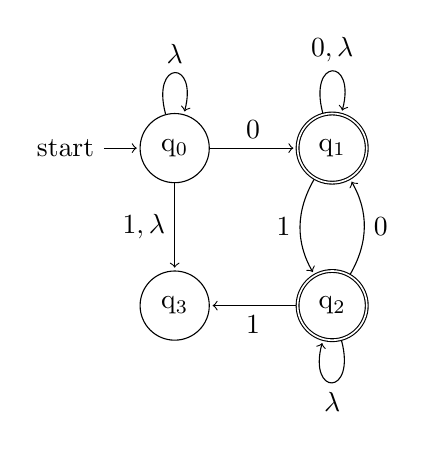
\begin{tikzpicture}[shorten >=1pt, node distance=2cm, on grid, auto][h]
  \node[state, initial] (q0) {$\mathrm{q}_{0}$};
  \node[state, accepting] (q1) [right=of q0] {$\mathrm{q}_{1}$};
  \node[state, accepting] (q2) [below of=q1] {$\mathrm{q}_{2}$};
  \node[state] (q3) [below of=q0] {$\mathrm{q}_{3}$};

  \path[->]
  (q0) edge node {0} (q1)
    (q0) edge[loop above] node {$\lambda$} (q0)
    (q0) edge node[left] {$1,\lambda$} (q3)
  (q1) edge[loop above] node {$0, \lambda$} (q1)
    (q1) edge[bend right] node[left] {1} (q2)
  (q2) edge[bend right] node[right] {0} (q1)
    (q2) edge node{1} (q3)
    (q2) edge[loop below] node {$\lambda$} (q2);
\end{tikzpicture}
}

% Cau 2
\qs{Answer the following question}{
For the $\lambda - \mathrm{NFA}$\\
Construct the equaivalent NFA.
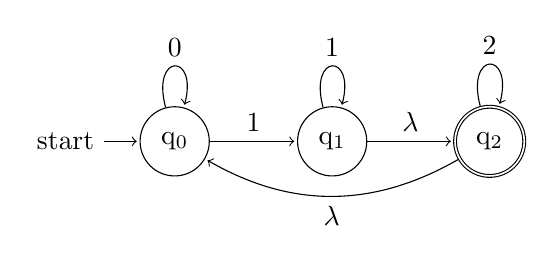
\begin{tikzpicture}[shorten >=1pt, node distance=2cm, on grid, auto][h]
  \node[state, initial] (q0) {$\mathrm{q}_{0}$};
  \node[state] (q1) [right=of q0] {$\mathrm{q}_{1}$};
  \node[state, accepting] (q2) [right=of q1] {$\mathrm{q}_{2}$};

  \path[->]
  (q0) edge node {1} (q1)
    (q0) edge[loop above] node {0} (q0)
  (q1) edge[loop above] node {1} (q1)
    (q1) edge node {$\lambda$} (q2)
  (q2) edge[loop above] node {2} (q2)
    (q2) edge[bend left, below] node{$\lambda$} (q0);
\end{tikzpicture}
\newline
}

\sol{\newline
Let us define the above $\lambda - \mathrm{NFA}$ as $M=\left(\{q_0, q_1, q_2\},\{0,1,2\}, \delta, \{ q_2 \}\right)$.\\
Moreover, define the NFA as $N = (Q', \sum, \delta', q', \mathds{F}')$:\\
1. $Q' = \{q_0, q_1, q_2\}$.\\
2. $\sum = \{ 0,1,2 \}$.\\
3. $q' = \{ q_0 \}$.\\
4. $\mathds{F}' = \{ q_0, q_2 \}$.\\
Since we know that  $ \delta'(q, a)= \hat{\delta}(q, a)$. Hence, we obtain the following state transitions.\\
First, we obtain the lambda closure:
\begin{itemize}
  \item $\lambda - \mathrm{closure}(q_0) = \{ q_0 \}$
  \item $\lambda - \mathrm{closure}(q_1) = \{ q_0, q_1, q_2 \}$
  \item $\lambda - \mathrm{closure}(q_2) = \{ q_0, q_2 \}$
\end{itemize}
(see next page)
}
% \newline

\pagebreak
\noindent $\delta'(q_0,0) = \hat{\delta}(q_0,0) = \delta(\lambda-\mathrm{closure}(q_0),0) = \delta(\{ q_0 \},0) = \{ q_0 \}$\\
$\delta'(q_0,1) = \hat{\delta}(q_0,1) = \delta(\lambda-\mathrm{closure}(q_0),1) = \delta(\{ q_0 \},1) = \{ q_0, q_1, q_2 \}$\\
$\delta'(q_0,2) = \hat{\delta}(q_0,2) = \delta(\lambda-\mathrm{closure}(q_0),2) = \delta(\{ q_0 \},2) = \{ \emptyset \}$\\
$\delta'(q_1,0) = \hat{\delta}(q_1,0) = \delta(\lambda-\mathrm{closure}(q_1),0) = \delta(\{ q_0, q_1, q_2 \},0) = \{ q_0 \}$\\
$\delta'(q_1,1) = \hat{\delta}(q_1,1) = \delta(\lambda-\mathrm{closure}(q_1),1) = \delta(\{ q_0, q_1, q_2 \},1) = \{ q_0, q_1, q_2 \}$\\
$\delta'(q_1,2) = \hat{\delta}(q_1,2) = \delta(\lambda-\mathrm{closure}(q_1),2) = \delta(\{ q_0, q_1, q_2 \},2) = \{ q_0, q_2 \}$\\
$\delta'(q_2,0) = \hat{\delta}(q_2,0) = \delta(\lambda-\mathrm{closure}(q_2),0) = \delta(\{ q_0, q_2 \},0) = \{ q_0 \}$\\
$\delta'(q_2,1) = \hat{\delta}(q_2,1) = \delta(\lambda-\mathrm{closure}(q_2),1) = \delta(\{ q_0, q_2 \},1) = \{ q_0, q_1, q_2 \}$\\
$\delta'(q_2,2) = \hat{\delta}(q_2,2) = \delta(\lambda-\mathrm{closure}(q_2),2) = \delta(\{ q_0, q_2 \},2) = \{ q_0, q_2 \}$\\

\textbf{State transition table}:
\begin{table}[H]
  \centering
  \begin{tabular}{|c|c|c|c|}
  \hline
  $\delta'$ & 0        & 1                      & 2                            \\ \hline
  $q_0$                   & $\{q_0\}$ & $\{ q_0, q_1, q_2 \}$ & $\{\emptyset\}$ \\ \hline
  $q_1 $                  & $\{q_0\}$ & $\{ q_0, q_1, q_2 \}$ & $\{ q_0, q_2 \}$            \\ \hline
  $q_2 $                  & $\{q_0\}$ & $\{ q_0, q_1, q_2 \}$ & $\{ q_0, q_2 \}$            \\ \hline
  \end{tabular}
\caption{NFA's state transition table}
\end{table}
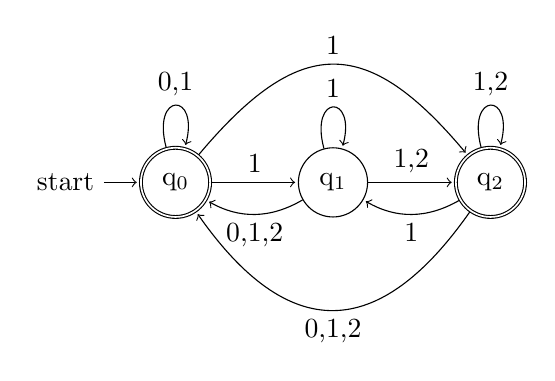
\begin{tikzpicture}[shorten >=1pt, node distance=2cm, on grid, auto][h]
  \node[state, initial, accepting] (q0) {$\mathrm{q}_{0}$};
  \node[state] (q1) [right=of q0] {$\mathrm{q}_{1}$};
  \node[state, accepting] (q2) [right=of q1] {$\mathrm{q}_{2}$};

  \path[->]
  (q0) edge[loop above] node {0,1} (q0)
    (q0) edge node {1} (q1)
    (q0) edge[bend left=50, looseness=1.5] node {1} (q2)
  (q1) edge[bend left] node {0,1,2} (q0)
    (q1) edge[loop above] node {1} (q1)
    (q1) edge node {1,2} (q2)
  (q2) edge[bend left=55, looseness=1.5] node {0,1,2} (q0)
    (q2) edge[bend left] node {1} (q1)
    (q2) edge[loop above] node {1,2} (q2);  
\end{tikzpicture}
\newline

% Cau 3
\qs{Answer the following question}{
Construct three $\lambda$-NFA's equivalent to the following regular expression:\\
  a. $10+(0+11) 0^* 1$\\
  b. $01\left[\left((10)^*+111\right)^*+0\right]^* 1$\\
  c. $01^* 0+01^* 10^*+1^* 0^*$
}

\sol{\newline
a.\newline
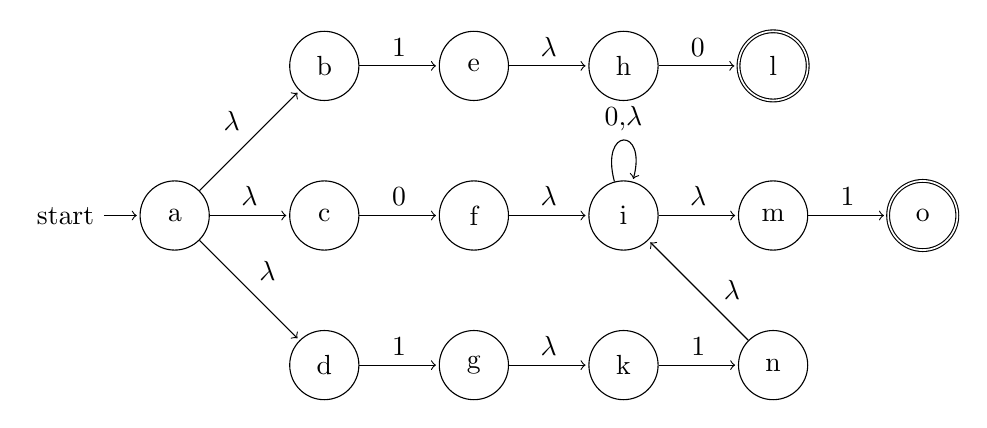
\begin{tikzpicture}[shorten >=1pt, node distance=1.9cm, on grid, auto][h]
  \node[state, initial] (a) {a};
  \node[state] (c) [right=of a] {c};
  \node[state] (b) [above of=c] {b};
  \node[state] (d) [below of=c] {d};
  \node[state] (e) [right=of b] {e};
  \node[state] (f) [right=of c] {f};
  \node[state] (g) [right=of d] {g};
  \node[state] (h) [right=of e] {h};
  \node[state] (i) [right=of f] {i};
  \node[state] (k) [right=of g] {k};
  \node[state, accepting] (l) [right=of h] {l};
  \node[state] (m) [right=of i] {m};
  \node[state] (n) [right=of k] {n};
  \node[state, accepting] (o) [right=of m] {o};

  \path[->]
  (a) edge node {$\lambda$} (b)
    (a) edge node {$\lambda$} (c)
    (a) edge node {$\lambda$} (d)
  (b) edge node {1} (e)
  (c) edge node {0} (f)
  (d) edge node {1} (g)
  (e) edge node {$\lambda$} (h)
  (f) edge node {$\lambda$} (i)
  (g) edge node {$\lambda$} (k)
  (h) edge node {0} (l)
  (i) edge[loop above] node {0,$\lambda$} (i)
    (i) edge node {$\lambda$} (m)
  (k) edge node {1} (n)
  (m) edge node {1} (o)
  (n) edge node[right=0.2] {$\lambda$} (i);
\end{tikzpicture}

\noindent (see next page for b. and c.)

\pagebreak

\noindent b. \newline
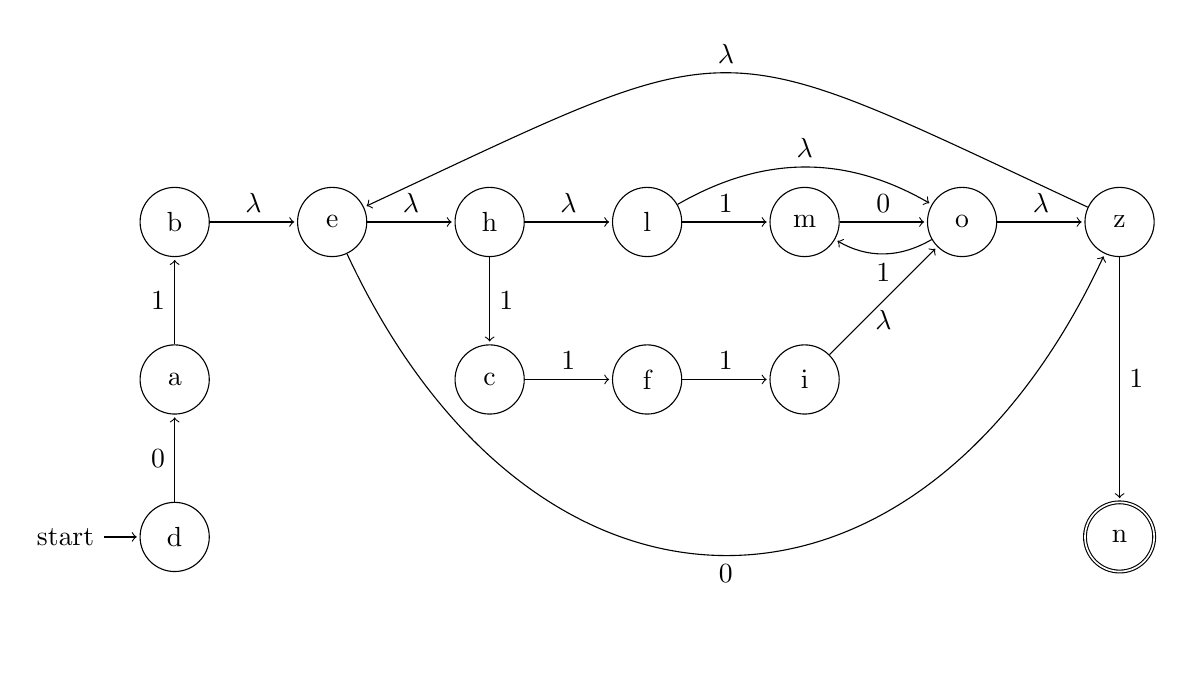
\begin{tikzpicture}[shorten >=1pt, node distance=2cm, on grid, auto]
  \node[state] (a) {a};
  \node[state] (b) [above of=a] {b};
  \node[state, initial] (d) [below of=a] {d};
  \node[state] (e) [right=of b] {e};
  \node[state] (h) [right=of e] {h};
  \node[state] (c) [below of=h] {c};
  % \node[state] (g) [below=4cm of e] {g};
  \node[state] (f) [right=of c] {f};
  \node[state] (i) [right=of f] {i};
  \node[state] (l) [right=of h] {l};
  \node[state] (m) [right=of l] {m};
  \node[state] (o) [right=of m] {o};
  \node[state] (z) [right=of o] {z};
  % \node[state] (k) [below=4cm of z] {k}; 
  \node[state, accepting] (n) [below=4cm of z] {n};  

  \path[->]
  (d) edge node {0} (a)
  (a) edge node {1} (b)
  (b) edge node {$\lambda$} (e)
  (e) edge node {$\lambda$} (h)
  (h) edge node {$\lambda$} (l)
  (l) edge node {1} (m)
    (l) edge[above, bend left] node {$\lambda$} (o)
  (m) edge node {0} (o)
  (o) edge node {$\lambda$} (z)
    (o) edge[below, bend left] node {1} (m)
  (z) edge[above, bend right=25, looseness=1.5] node {$\lambda$} (e)
  (h) edge node {1} (c)
  (c) edge node {1} (f)
  (f) edge node {1} (i)
  (i) edge node[below] {$\lambda$} (o)
  % (z) edge node {$\lambda$} (k)
  % (k) edge node {1} (n)
  % (k) edge[below, bend left=40, looseness=1.5] node {$\lambda$} (b)
  % (e) edge[bend right] node {0} (g)
  (z) edge node {1} (n)
  (e) edge[bend right=65, looseness=1.5, below] node {0} (z);
  % (g) edge node {$\lambda$} (k);
\end{tikzpicture}
\newline

\noindent c.\newline
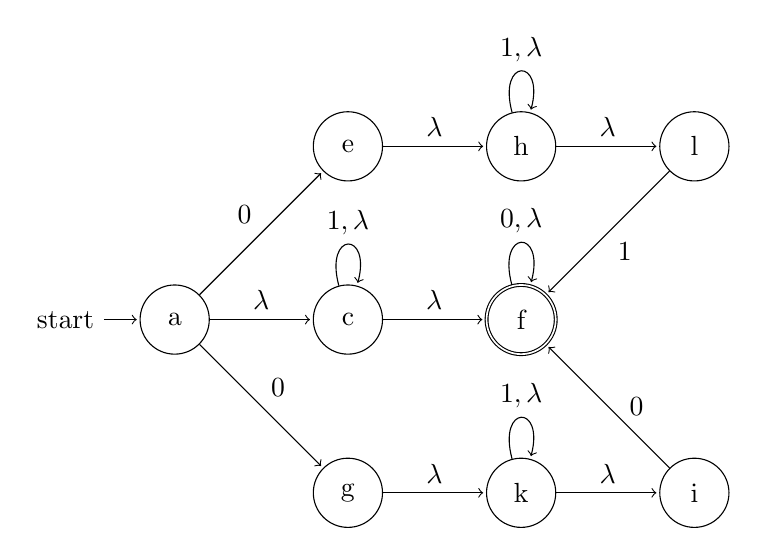
\begin{tikzpicture}[shorten >=1pt, node distance=2.2cm, on grid, auto][h]
  \node[state, initial] (a) {a};
  \node[state] (c) [right=of a] {c};
  % \node[state] (b) [above of=a] {b};
  % \node[state] (d) [below of=a] {d};
  \node[state] (e) [above of=c] {e};
  \node[state, accepting] (f) [right=of c] {f};
  \node[state] (g) [below of=c] {g};
  \node[state] (h) [right=of e] {h};
  \node[state] (k) [right=of g] {k};
  \node[state] (i) [right=of k] {i};
  \node[state] (l) [right=of h] {l};
  % \node[state] (m) [right=of f] {m};

  \path[->]
  (a) edge node {0} (e)
    (a) edge node {$\lambda$} (c)
    (a) edge node {0} (g)
  (c) edge[loop above] node {$1, \lambda$} (c)
    (c) edge node {$\lambda$} (f)
  (f) edge[loop above] node {$0,\lambda$} (f)
  % (d) edge node {0} (g)
  (g) edge node {$\lambda$} (k)
  (k) edge[loop above] node {$1,\lambda$} (k)
    (k) edge node {$\lambda$} (i)
  (i) edge node[right=0.15] {0} (f)
  % (b) edge node {0} (e)
  (e) edge node {$\lambda$} (h)
  (h) edge[loop above] node {$1,\lambda$} (h)
    (h) edge node {$\lambda$} (l)
  (l) edge node {1} (f);
\end{tikzpicture}

\noindent This is the most optimized approach that I could possibly get. :D
} %011101000111000
\end{document}
